\documentclass{article}
\usepackage[letterpaper, portrait, margin=0.2in]{geometry}
\usepackage{rtex}
\usepackage{enumitem}
\usepackage{minted}
\usepackage{fontspec}
\setmonofont{Jetbrains Mono}
\usepackage[fontsize=7pt]{fontsize}

\newcommand{\scinot}[1]{\times 10^{#1}}

\begin{document}

\begin{multicols*}{4}
  \formbox{Ideal Diode Definition}{
    \begin{center}
      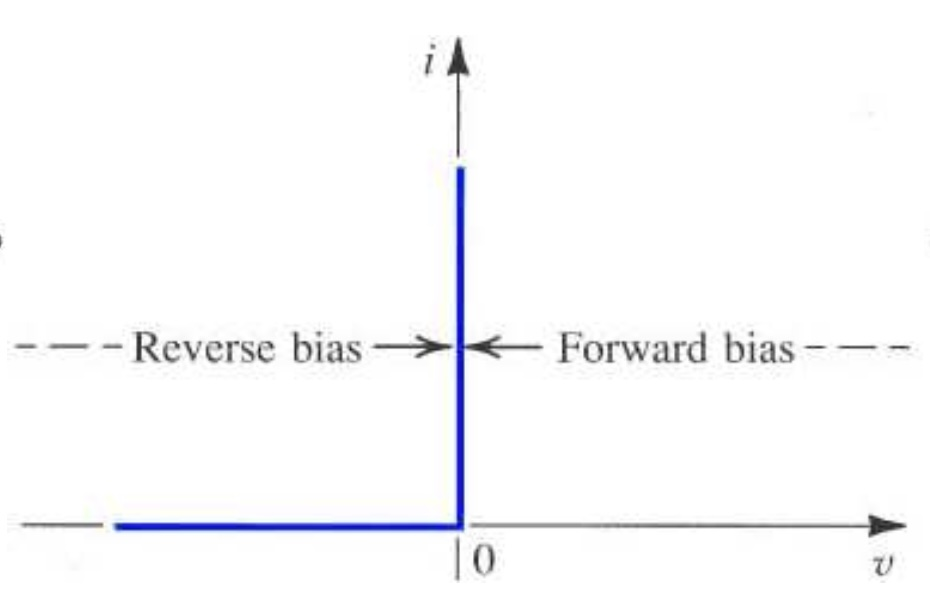
\includegraphics[width=\textwidth]{images/ideal_diode.jpg}
    \end{center}
  }
  \formbox{DC Diode Analysis}{Either know voltages and treat as open/short circuits, or
    guess and check.}
  \formbox{Basic Half Rectifier}{\begin{center}
      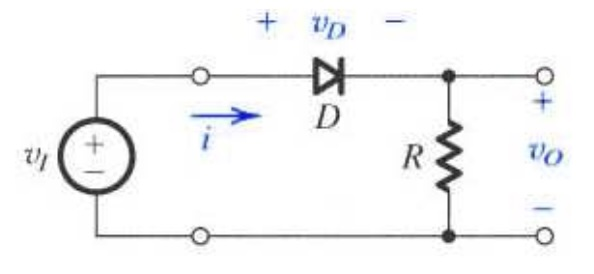
\includegraphics[width=\textwidth]{images/half_rectifier.jpg}
    \end{center}
  }
  \formbox{Ideal Diode Rectifier\\Conduction Angle}{
    \begin{align*}
      2\theta = 2\cos^{-1} \left(\frac{V_S^{\text{fwd}}}{V_S^\text{amp}}\right)
    \end{align*}
  }
  \formbox{Seleting Peak Inverse Voltage}{
    \begin{align*}
      \text{PIV}_\text{des} = 1.5\text{PIV}
    \end{align*}
  }
  \formbox{Real Diode}{
    \begin{center}
      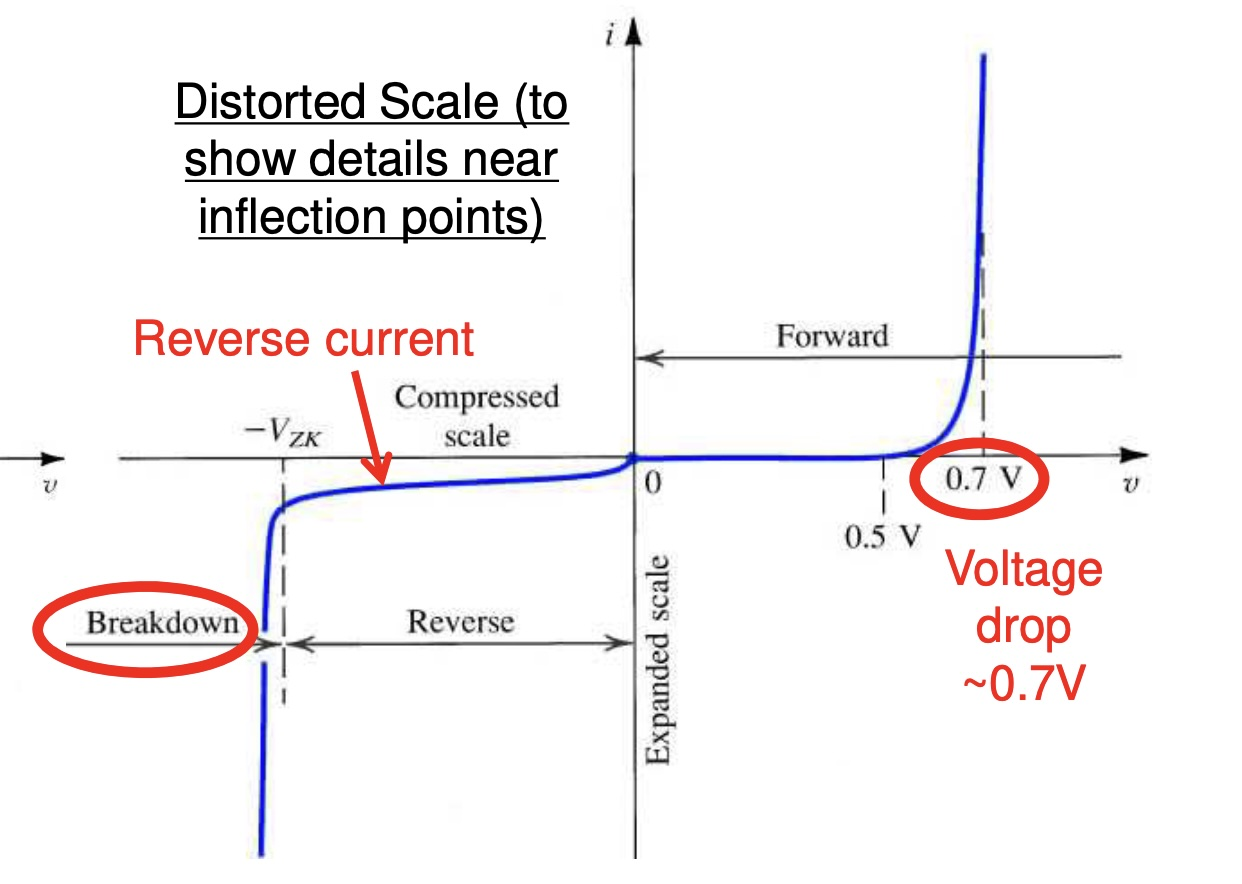
\includegraphics[width=\textwidth]{images/real_diode.jpg}
    \end{center}
  }
  \formbox{Real Diode Model}{
    \begin{align*}
      i &= I_S \left(\exp(\frac{v}{nV_T}) - 1\right)\\
      V_T &= \frac{kT}{q}
    \end{align*}
    $n=1$, $k = 1.38\cdot 10^{-23} \text{J}/\text{K}$, $q = 1.602 \cdot 10^{-19} \text{C}$,
    $T = 300\text{K}$.
  }
  \formbox{Simplified Diode Model}{
    For $i \gg I_S$ or $v > 10 nV_T$:
    \begin{align*}
      i \approxeq I_Se^{v/nV_T}
    \end{align*}
  }
  \formbox{Zener Diode}{
    \begin{center}
      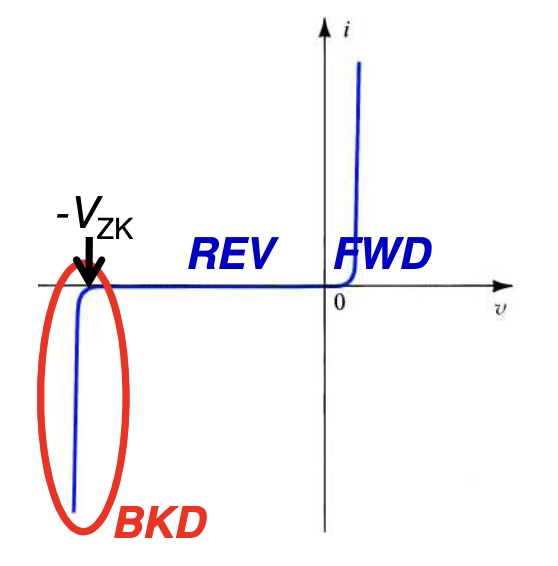
\includegraphics[width=\textwidth]{images/zener.jpg}
    \end{center}
    Knee current is the min current at breakdown.
  }
  \formbox{Iterative Analysis for Diodes}{
    \begin{center}
      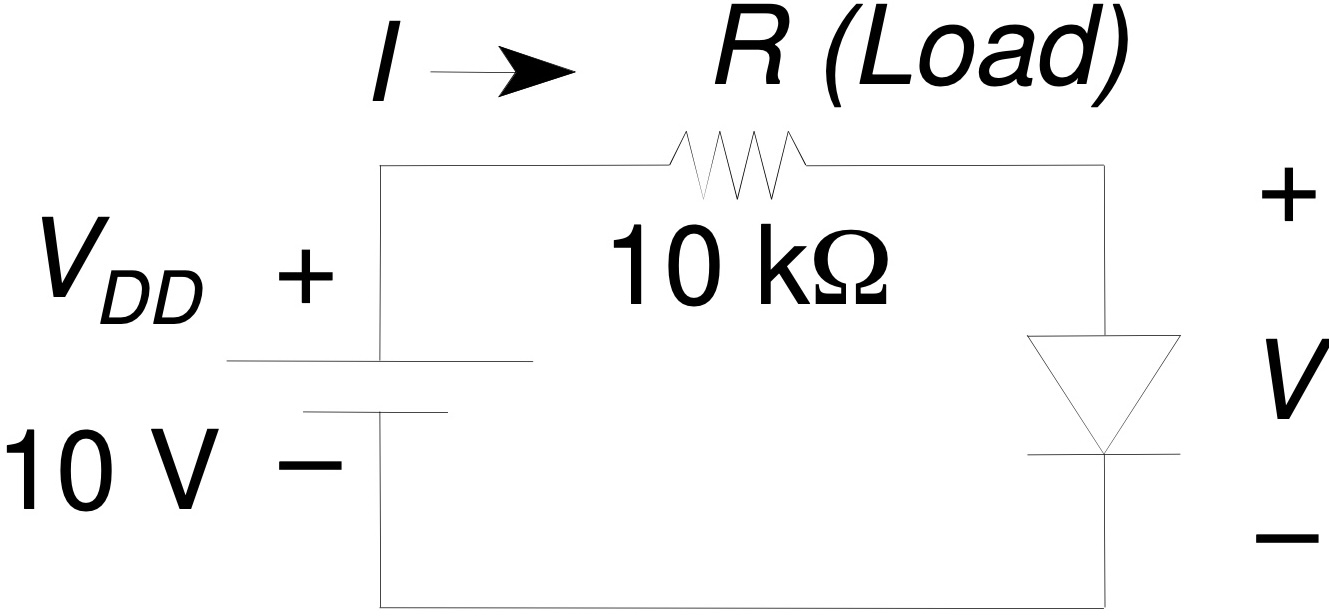
\includegraphics[width=\textwidth]{images/iterative_circuit.jpg}
    \end{center}
    \begin{align}
      V_\text{DD} &= IR + V\\
      I &= I_S(e^{V/V_T} - 1)\\
      I_S &\approxeq x e^{-0.7 / V_T}
    \end{align}
    \begin{enumerate}[label=\alph*., leftmargin=1.5em, labelsep=0.5em, itemsep=-0.2em]
    \item Using your guess for $V$, calculate $I$ from (1).
    \item Substitute $I$ into (2) to get a new value for $V$.
    \item Substitute $V$ back into (1) to get a value for $I$.
    \end{enumerate}
    Continue iterating until:
    \begin{align*}
      \frac{(I_n - I_{n - 1})}{I_n} \leq 1\%
    \end{align*}
  }
  \formbox{Zener Approximation in BKD}{
    $V_Z = V_{Z0} + r_Z I_Z$
    \begin{center}
      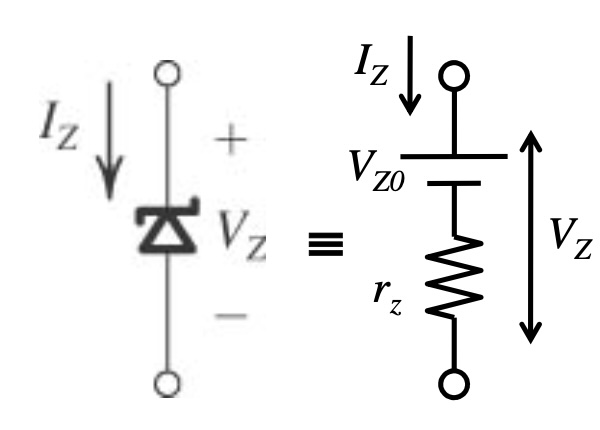
\includegraphics[width=\textwidth]{images/zener_approx.jpg}
    \end{center}
  }
  \formbox{Zener Regulators}{
    \begin{center}
      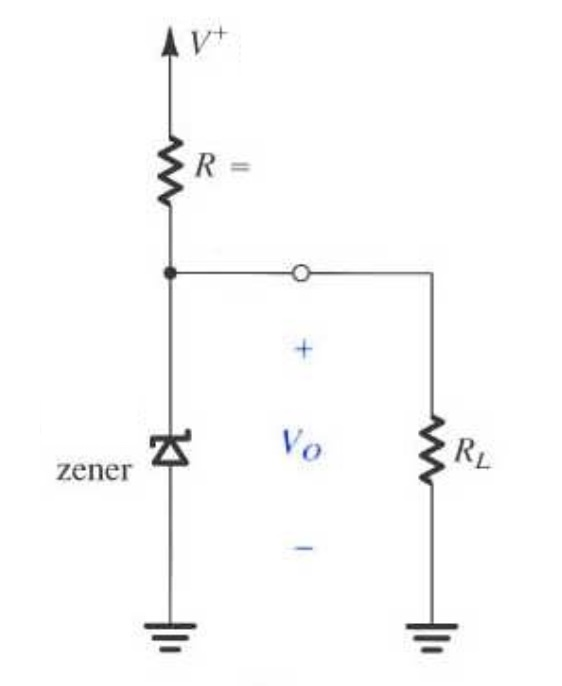
\includegraphics[width=0.6\textwidth]{images/zener_regulator.jpeg}
    \end{center}
    \begin{align*}
      V_0 &= V_{Z0} \frac{\frac{R}{R_L}}{r_Z + \frac{R}{R_L}} \\&\,\,\,\, + V^+ \frac{\frac{r_Z}{R_L}}{R + \frac{r_Z}{R_L}}\\
      \Delta V_0 &= \Delta V^+ \frac{\frac{R_L}{r_z}}{R + \frac{R_L}{r_z}}\\
      V_0 &= V_{Z0} + \frac{V^+ - V_0}{R}r_z
    \end{align*}    
  }
  \formbox{Line Regulation}{  \begin{align*}
    \eval{\frac{\Delta V_0}{\Delta V^+}}_{I_L=\text{constant}} = \frac{r_Z}{R + r_Z}
  \end{align*}}
  \formbox{Load Regulation}{  \begin{align*}
    \eval{\frac{\Delta V_0}{\Delta I_L}}_{V^+ = \text{constant}} = - \frac{r_Z}{R}
  \end{align*}}
  \formbox{Supply Time Plot}{
    \begin{center}
      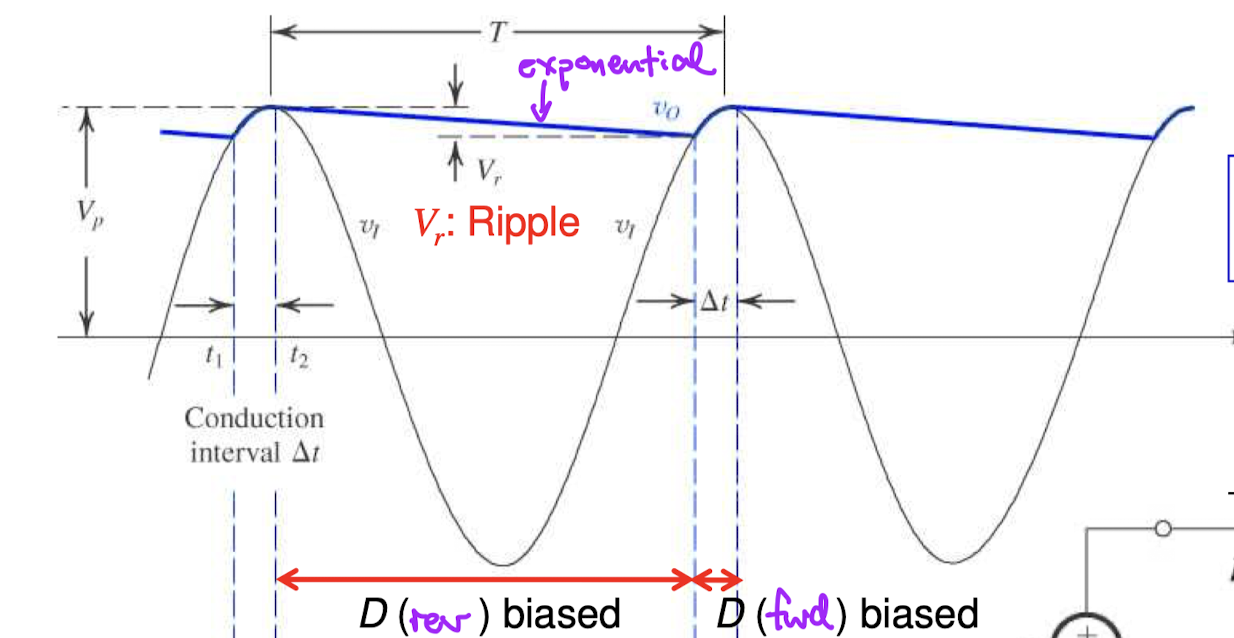
\includegraphics[width=\textwidth]{images/supply_time.png}
    \end{center}
  }
  \formbox{Ripple Voltage -- Full Rectifier}{
    \begin{align*}
      V_r \approxeq \frac{V_p T}{2 R_L C} = \frac{V_p}{2fR_L C}
    \end{align*}
  }
  
  \formbox{Ripple Voltage -- Half Rectifier}{
    \begin{align*}
      V_r \approxeq \frac{V_p T}{R_L C} = \frac{V_p}{fR_L C}
    \end{align*}
  }
  
  \formbox{Input Voltage}{    
    \begin{align*}
      V_p &\approxeq V_o = V_p - \frac{1}{2}V_r \approx V_p\\
      &\approxeq V_p \left(\frac{4fR_LC - 1}{4fR_LC}\right)
  \end{align*}}
  \formbox{Load Current}{
    \begin{align*}
      I_L &\approxeq \frac{R_L}{V_L} = \frac{V_p - \frac{1}{2}V_r}{R_L} \approx \frac{V_p}{R_L}
  \end{align*}}
  \formbox{Half Rectifier Average Output Voltage}{
    \begin{align*}
      V_o^\text{avg} = V_p - V_\text{D} - \frac{1}{2}V_r
    \end{align*}
  }
  \formbox{Conduction Angle}{
  \begin{align*}
    \omega \Delta t = \sqrt{\frac{2V_r}{V_p}}
  \end{align*}}
  \formbox{Max Diode Current}{
    \begin{align*}
      i_D^\text{max} \approxeq I_L\left(1 + 2\pi \sqrt{\frac{2V_p}{V_r}}\right)
  \end{align*}}
  \formbox{Average Diode Current}{
  \begin{align*}
    i_D^\text{ave} \approxeq I_L\left(1 + \pi \sqrt{\frac{2V_p}{V_r}}\right)
  \end{align*}}
  \formbox{Peak Inverse Voltage 2-Diode}{
  \begin{align*}
    PIV = 2V_p
  \end{align*}}
  \formbox{Peak Inverse Voltage 4-Diode}{
  \begin{align*}
    PIV = V_p
  \end{align*}}


  \formbox{Average Voltage}{You just have to integrate and divide by the total period ($2\pi$).}

  \formbox{FULL BRIDGE RECTIFIER}{
    \begin{center}
      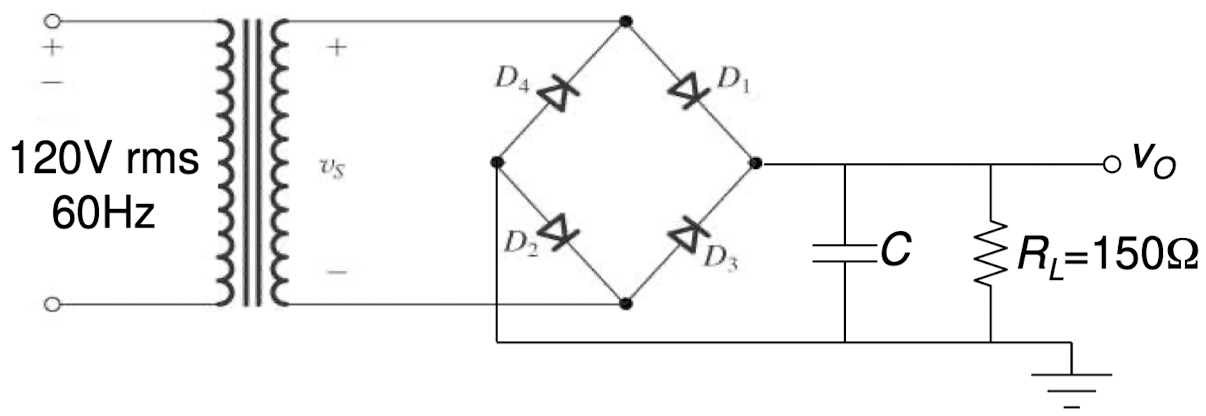
\includegraphics[width=\textwidth]{images/bridge_rectifier.png}
    \end{center}
  }

  \formbox{Peak Voltage for Bridge Supply}{
    \begin{align*}
      V_\text{max} &= V_p - 2 V_d
    \end{align*}
  }

  \formbox{Conduction Time Fraction}{
    \begin{align*}
      \tau = \frac{\pi - 2\theta}{2\pi}      
    \end{align*}
  }
  
  \formbox{Substitutions for Real Case Constant Voltage Drop}{
Half-Wave
  \begin{align*}
    V_p &\to V_p - V_D\\
    PIV &= 2V_p - V_D \\
    &= (V_p - V_D) - (- V_p)
  \end{align*}
Full-Wave
  \begin{align*}
    V_p &\to V_p - V_D \qquad \text{(2D)}\\
    V_p &\to V_p - 2V_D \qquad \text{(4D)}\\
    PIV &\approxeq 2V_p - V_D \qquad \text{(2D)}\\
    PIV &\approxeq V_p - V_D \qquad \text{(4D)}
  \end{align*}}
  \formbox{DC Restorer}{
  \begin{center}
    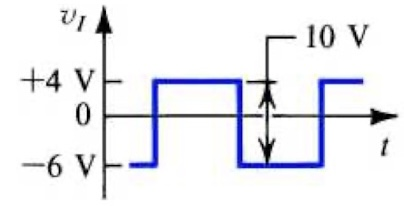
\includegraphics[width=0.65\textwidth]{images/dc_restorer_1.jpg}
    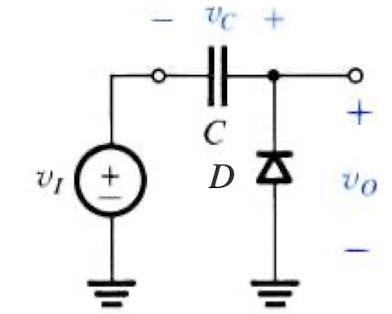
\includegraphics[width=0.5\textwidth]{images/dc_restorer_2.jpg}
    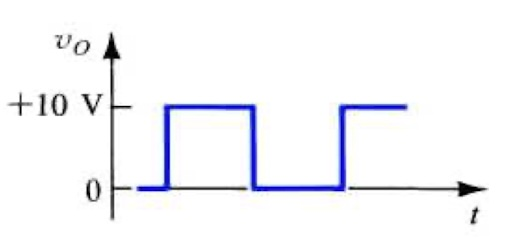
\includegraphics[width=0.65\textwidth]{images/dc_restorer_3.jpg}
  \end{center}
  Reversing the polarity of $D$ makes the signal negative.
  }
  \formbox{Voltage Doubler}{
    \begin{center}
      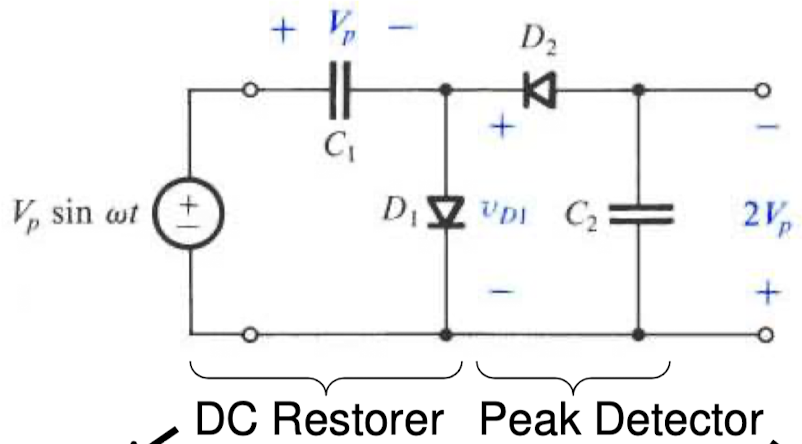
\includegraphics[width=\textwidth]{images/voltage_doubler_circuit.png}
      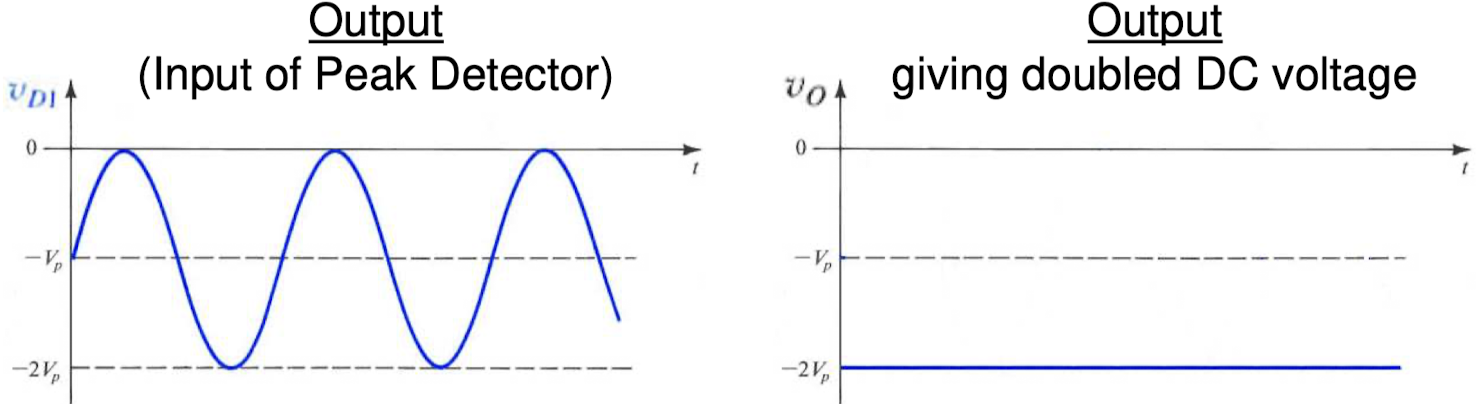
\includegraphics[width=\textwidth]{images/voltage_doubler_output.png}
    \end{center}
  }
  \formbox{Center-Tapped Rectifier}{
    \begin{center}
      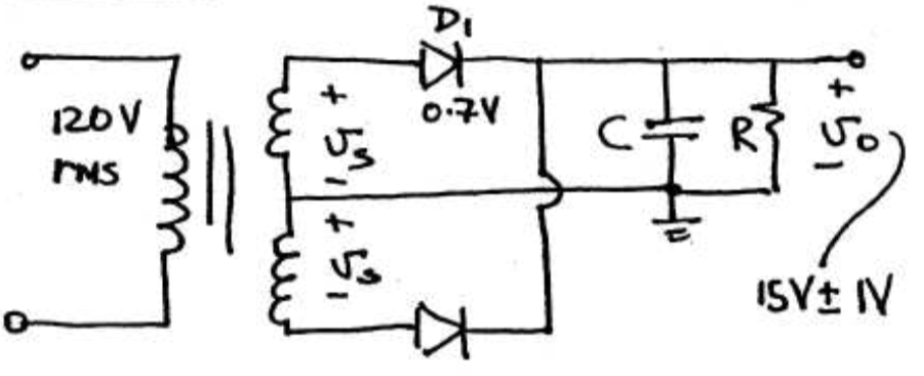
\includegraphics[width=\textwidth]{images/center_tapped.png}
    \end{center}
  }
  \formbox{Required Output Voltage for Supply}{
    \begin{align*}
      V_\text{req} = V_{o,\, \text{des}} + V_D + \Delta V_{o,\, \text{des}}
    \end{align*}
  }
  \formbox{Required Secondary RMS}{
    \begin{align*}
      V_p = \frac{n V_\text{req}}{\sqrt{2}}
    \end{align*}
    $n$ is the number of equispaced ``taps''.
  }

  \formbox{ree}{
    \begin{center}
      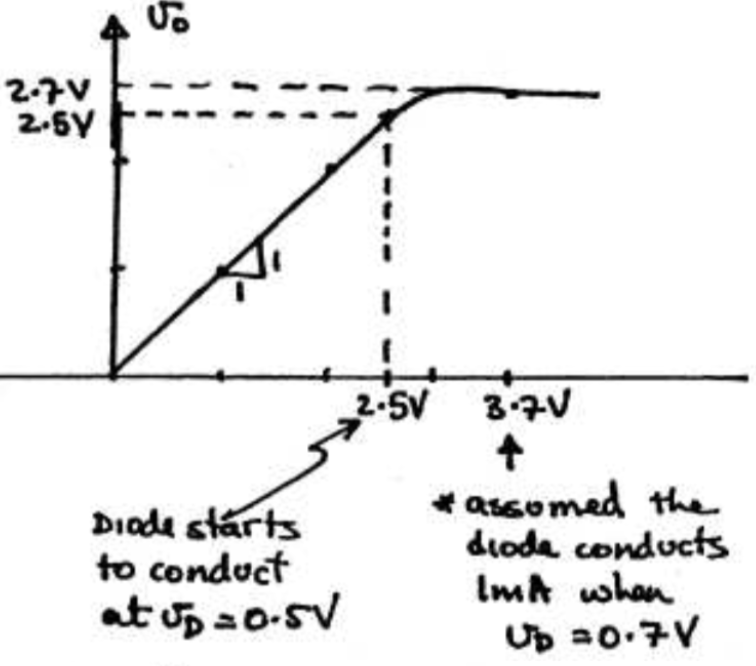
\includegraphics[width=0.75\textwidth]{images/ree.png}
    \end{center}
  }
  \formbox{Piecewise Linear Model}{
    \begin{center}
      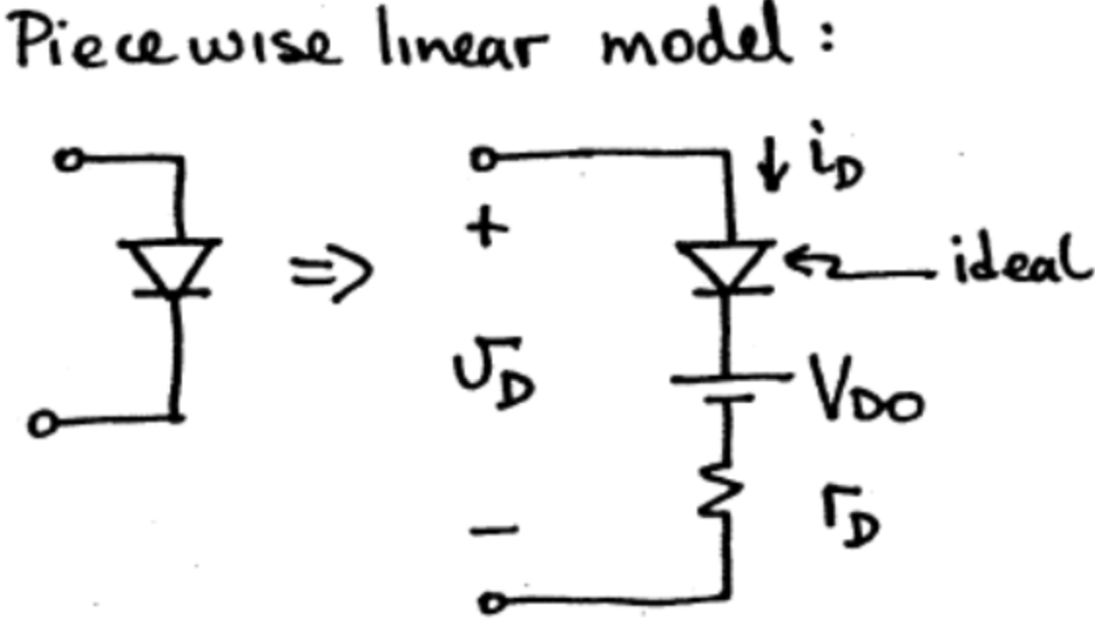
\includegraphics[width=\textwidth]{images/piecewise_linear_model.png}
    \end{center}
    Use the exponential model to find two points, and then $y=mx+b$.
  }
  \formbox{Clipping Circuit}{
    \begin{align*}
      v_o = 
      \begin{cases}
        L_+ & v_i > \frac{L_+}{K}\\
        Kv_i & \frac{L_-}{K} \leq v_i \leq \frac{L_+}{K}\\
        L_- & v_i < \frac{L_-}{K}
      \end{cases}
    \end{align*}
  }
  

\end{multicols*}

\pagebreak

\begin{multicols*}{3}
  \formbox{Intrinsic Carrier Concentration for Pure Silicon}{
    \centering
      $\ds n_i^2 = BT^3\exp\left(-\frac{E_g}{kT}\right)$\\
    \raggedright
    where:\\
    $E_g = 1.12$eV: band gap\\
    $T$: temperature\\
    $k = 8.62\times 10^{-5}$eV/K: Boltzmann constant\\
    $B = 5.4\times 10^{31}$
  }

  \formbox{Fraction of Ionized Atoms}{
    \begin{align*}
      \frac{n_i}{N}
    \end{align*}
  }


  \formbox{Conductivity}{
    \centering
    $\ds \sigma = q(p\mu_p + n \mu_n)$\\    
    \raggedright
    Where:\\
    $p$: Concentration of free holes\\
    $n$: Concentration of free electrons\\
    $\mu_p$: Mobility of holes \\(RT: 480cm$^2$/V$\cdot$s)\\
    $\mu_n$: Mobility of electrons \\(RT: 1350cm$^2$/V$\cdot$s)\\
    $q = 1.6\scinot{-19}$C: Electron charge
  }

  \formbox{Charge Neutrality Relationship}{
    \centering
      $\ds N_D + p = N_a + n$\\
    \raggedright
    $N_D$: Concentration of donor atoms\\
    $N_A$: Concentration of acceptor atoms
  }

  \formbox{Resistance}{
    \centering
    $R = \frac{\rho L}{A}$\\
    \raggedright
    where $\rho = \frac{1}{\sigma}$ (resistivity).
  }

  \formbox{Law of Mass Action}{
    \centering
      $\ds n_i^2 = pn$\\
    \raggedright
    Note: $n_i$ for silicon is generally \\$1.45\scinot{10}$cm$^{-3}$.
  }

  \formbox{Diffusion Current for Holes}{
    \begin{align*}
      J_{p, \text{diffn}} = -q D_p \frac{dp}{dx}      
    \end{align*}
    Where $D_p = 34$cm$^2$/s at 300K
  }

  \formbox{Diffusion Current for Electrons}{
    \begin{align*}
      J_{n, \text{diffn}} = -q D_n \frac{dn}{dx}
    \end{align*}
    Where $D_p = 12$cm$^2$/s at 300K
  }

  \formbox{Total Diffusion Current Density}{
    \begin{align*}
      J_\text{diffn} = J_{p, \text{diffn}} + J_{n, \text{diffn}}      
    \end{align*}
  }

  \formbox{Drift Current Density}{
    \begin{align*}
      J = \sigma E      
    \end{align*}
  }

  \formbox{Drift Current}{
    \begin{align*}
      I = \sigma E \cdot A
    \end{align*}
  }

  \formbox{Mobility-Diffusivity Relationship (Einstein)}{
    \begin{align*}
      \frac{D_n}{\mu_n} = \frac{D_p}{\mu_p} = V_T
    \end{align*}
    Where $V_T$ is thermal voltage.
  }

  \formbox{Drift Velocity}{$\ds v_{\text{drift}, p/n} = \mu_{p/n}E$}

  \formbox{Thermal Voltage}{
    \begin{align*}
      V_T = \frac{kT}{q}
    \end{align*}
    $k = 1.38\scinot{-23}$\\
    $q = 1.6\scinot{-19}$    
  }

  \formbox{Built-In Voltage}{
    \begin{align*}
      V_0 = V_T \ln \left(\frac{N_A N_D}{n_i^2} \right)
    \end{align*}
  }

  \formbox{Depletion Region Width}{
    \begin{align*}
      W_\text{dep} = \sqrt{\frac{2\varepsilon_s}{q} \left(\frac{1}{N_A} + \frac{1}{N_D}\right) (V_0 - V)}
    \end{align*}
    $\varepsilon_s = 1.04\scinot{-12}$F/cm (Dielectric constant of Si)
  }

  \formbox{Charge in a Junction}{
    \centering
      $\ds q_J = q N V$\\
    \raggedright
  }

  \formbox{Drift Current pt2}{
    \centering
      $\ds J_\text{drift} = qp\mu_p E + qn\mu_nE$\\
    \raggedright
  }

  \formbox{Concentration Relationships: Open Circuit}{
    \begin{align*}
      p_{p0} &= p_{n0}e^{\frac{V_0}{V_T}} & n_{n0} &= n_{p0}e^{\frac{V_0}{V_T}}
    \end{align*}
    \begin{center}
      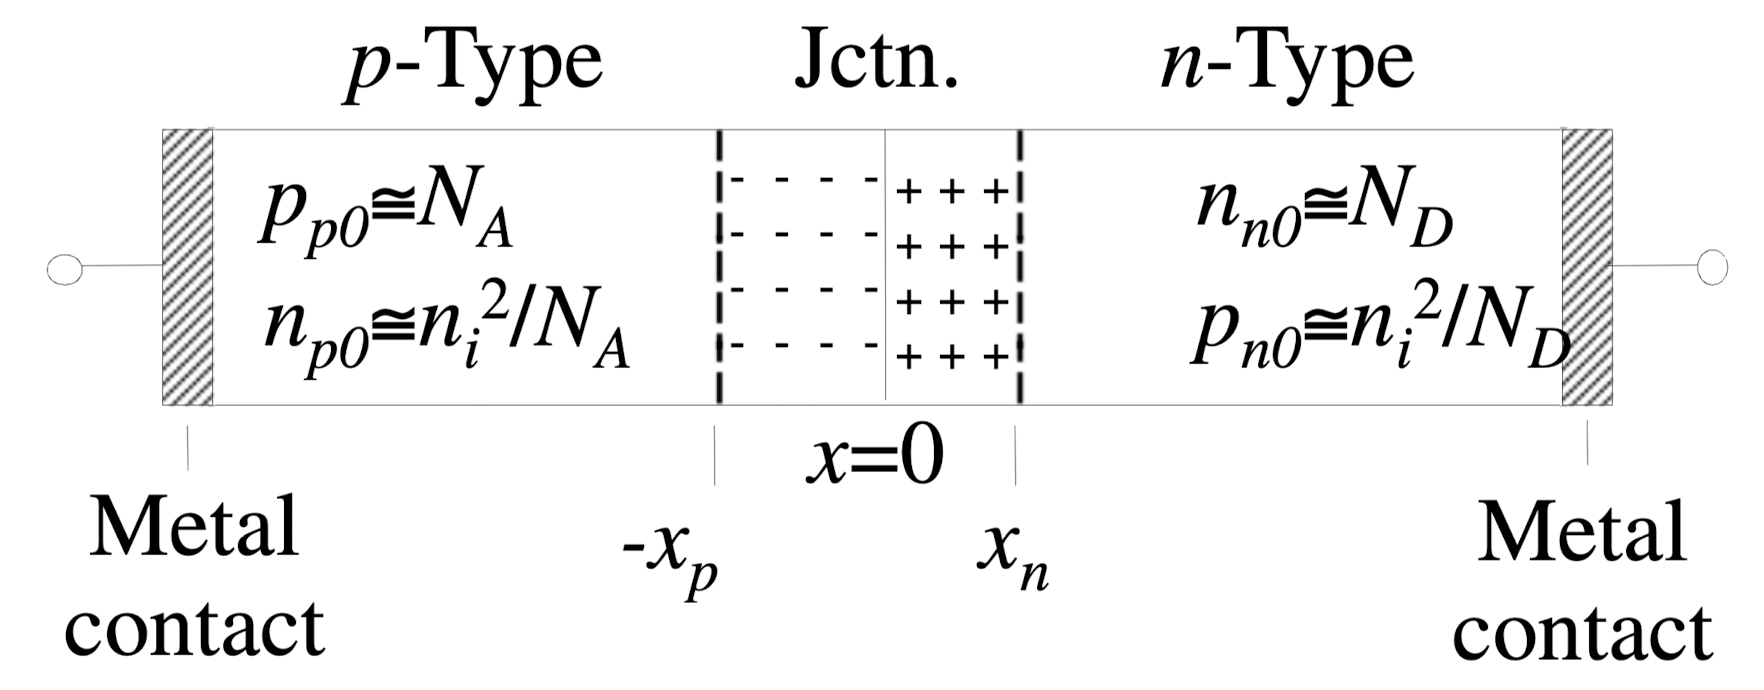
\includegraphics[width=\linewidth]{images/concentration_relationships.png}
    \end{center}
  }

  \formbox{Common Mode Rejection Ratio}{
    \begin{align*}
      \text{CMRR} = 20 \log \left(\frac{|A_d|}{|A_{cm}|}\right)
    \end{align*}    
  }

  \formbox{Op-Amp Golden Rules}{
    \begin{enumerate}
    \item Infinite Open Loop Gain ($A \to \infty$)
    \item No current flow through the inputs
    \item Potential difference between input pins is zero
    \end{enumerate}
  }

  \formbox{Weighted Summer}{
    \begin{center}
      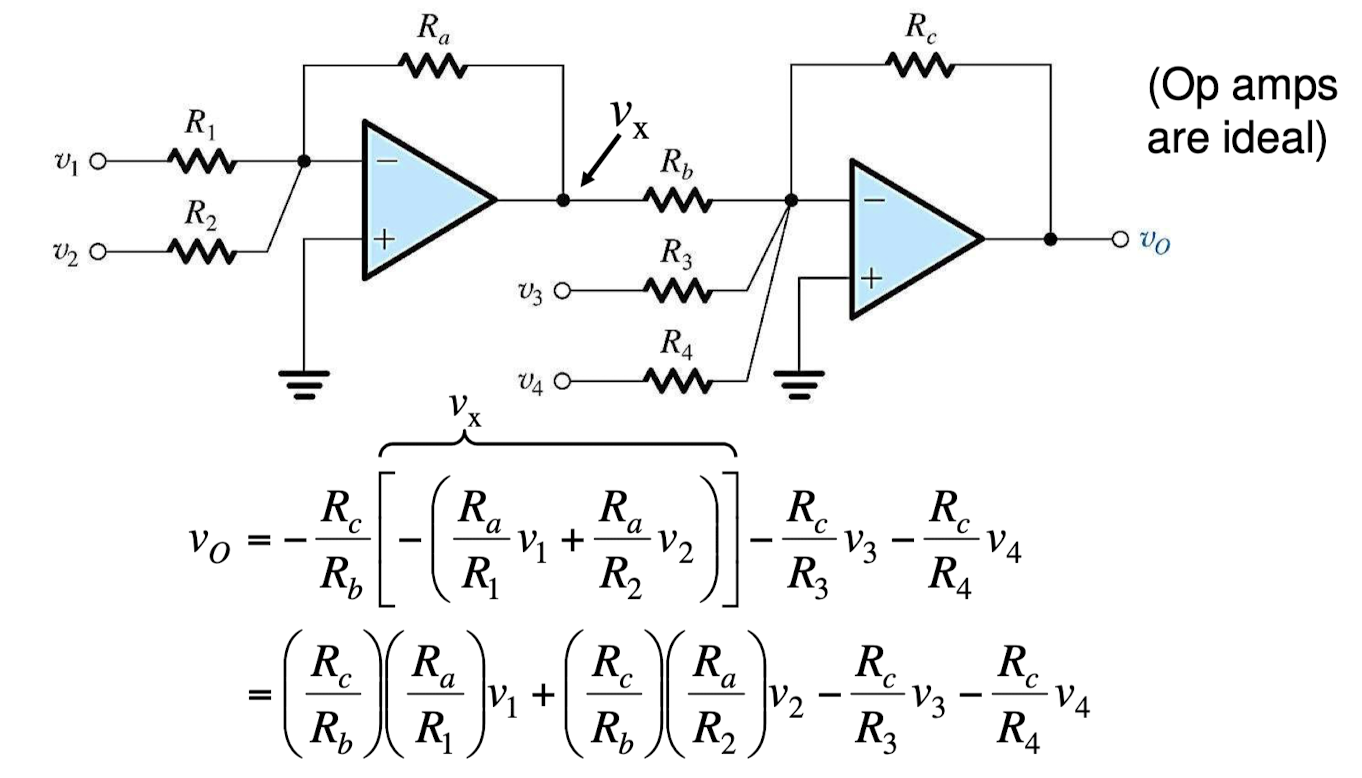
\includegraphics[width=\textwidth]{images/weighted_summer.png}
    \end{center}
  }

  \formbox{Inverting Amplifier}{
    \begin{center}
      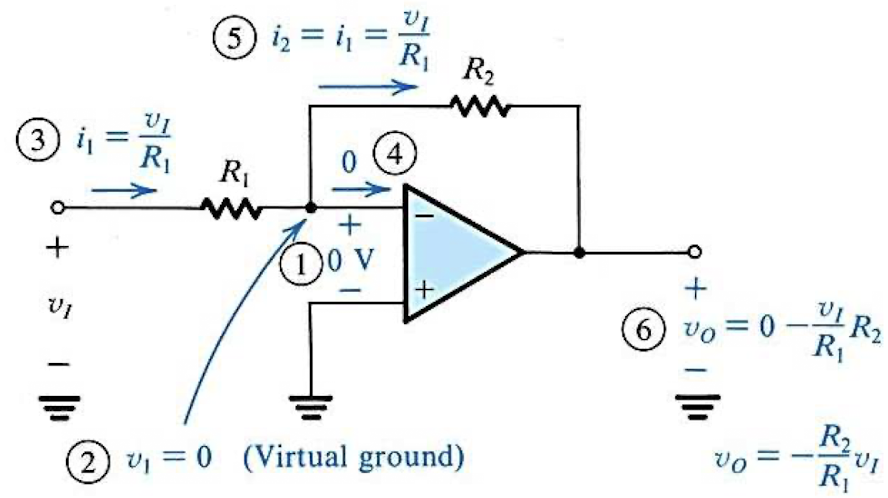
\includegraphics[width=\textwidth]{images/inverting_amplifier.png}
    \end{center}
  }

  \formbox{Non-Inverting Amplifier}{
    \begin{center}
      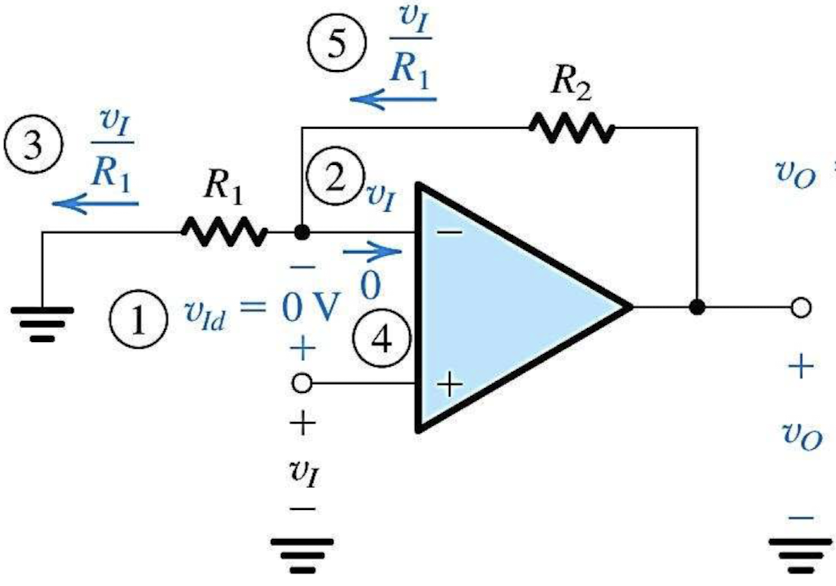
\includegraphics[width=0.7\textwidth]{images/non_inverting_amplifier.png}
    \end{center}
    $\ds G = 1 + \frac{R_2}{R_1}$
  }

  \formbox{Charge Density at Depletion Region}{
    \centering
    $\rho_p = -qN_A$ \qquad $\rho_n = qN_D$
  }
  \formbox{Charge Balancing}{
    \centering
    $qN_Ax_pA = qN_Dx_nA$ \quad or \quad $\frac{x_n}{x_p} = \frac{N_A}{N_D}$
  }
  \formbox{Depletion Zone Boundaries}{
    \centering
    $x_p = W_\text{dep} \frac{N_D}{N_A + N_D}$ \qquad $x_n = W_\text{dep}- x_p$
  }
  \formbox{Electric Field at Center of Depletion Zone}{
    \centering
    $\ds E(0) = -\frac{qN_A}{\varepsilon_S}x_p$    
  }
  \formbox{Differential Amplifier -- Common Mode Gain}{
    \centering
    $\ds A_{cm} = \frac{v_0}{v_{Icm}} = \left(\frac{R_4}{R_4 + R_3}\right) \left(1-\frac{R_2R_3}{R_1R_4}\right)$
    \\If ideal, can assume an error for $\frac{R_2R_3}{R_1R_4} = \gamma$ to calculate CMRR.
  }

  \formbox{Ideal Differential Amplifier}{
    \begin{center}
      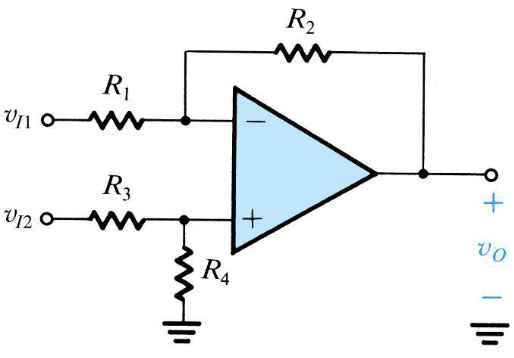
\includegraphics[width=0.7\textwidth]{images/ideal_diff_amp.png}
    \end{center}
    If $\ds \frac{R_4}{R_3} = \frac{R_2}{R_1}$ or $R_3 = R_1 \wedge R_4 = R_2$ then
    $\ds A_d = \frac{R_2}{R_1}$.
  }

  \formbox{Bistable Multivibrator}{
    \begin{center}
      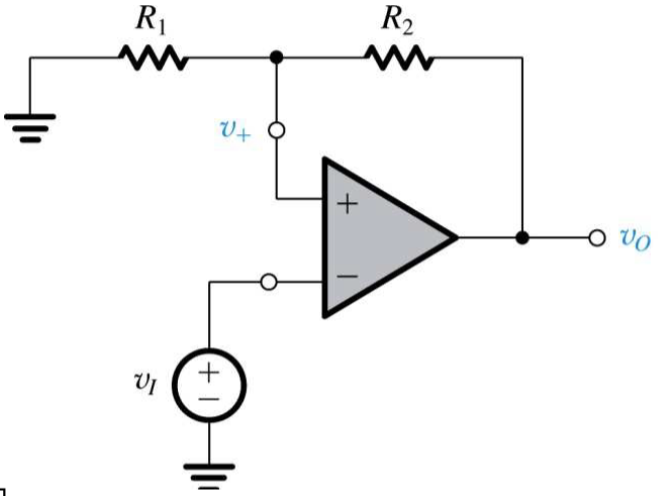
\includegraphics[width=0.6\textwidth]{images/multivibrator.png}
    \end{center}
  }

  \formbox{Hysterisis in Multivibrator Circuit}{
    \begin{center}
      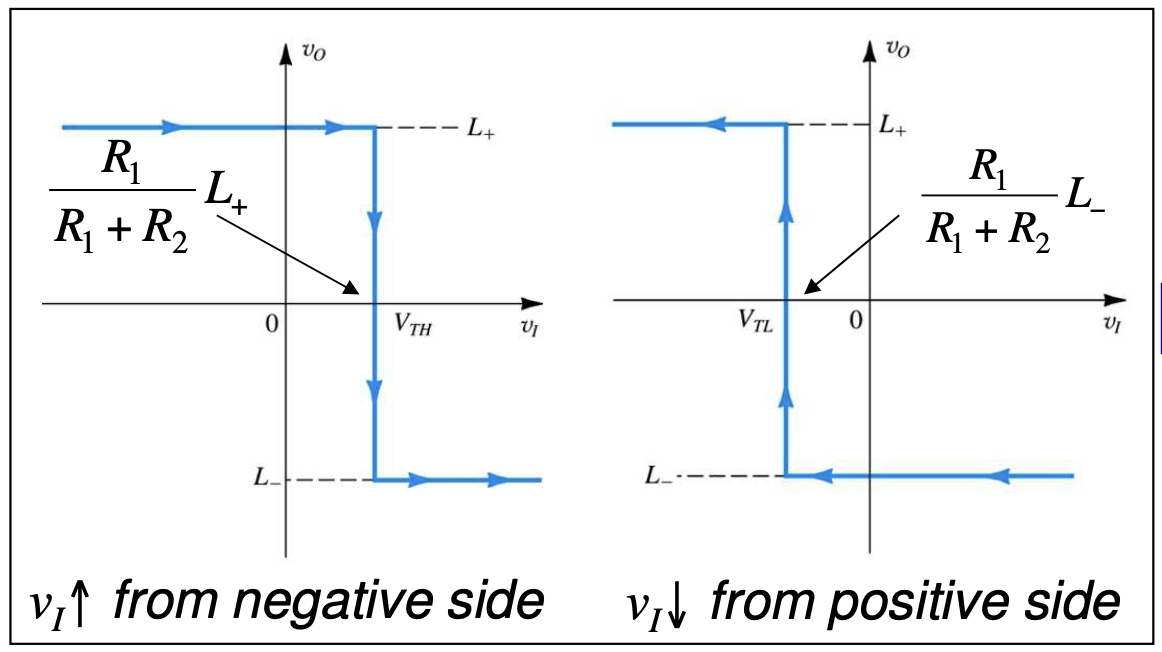
\includegraphics[width=\textwidth]{images/hysterisis.png}
    \end{center}
  }

  \formbox{Monostable Multivibrator}{
    \begin{center}
      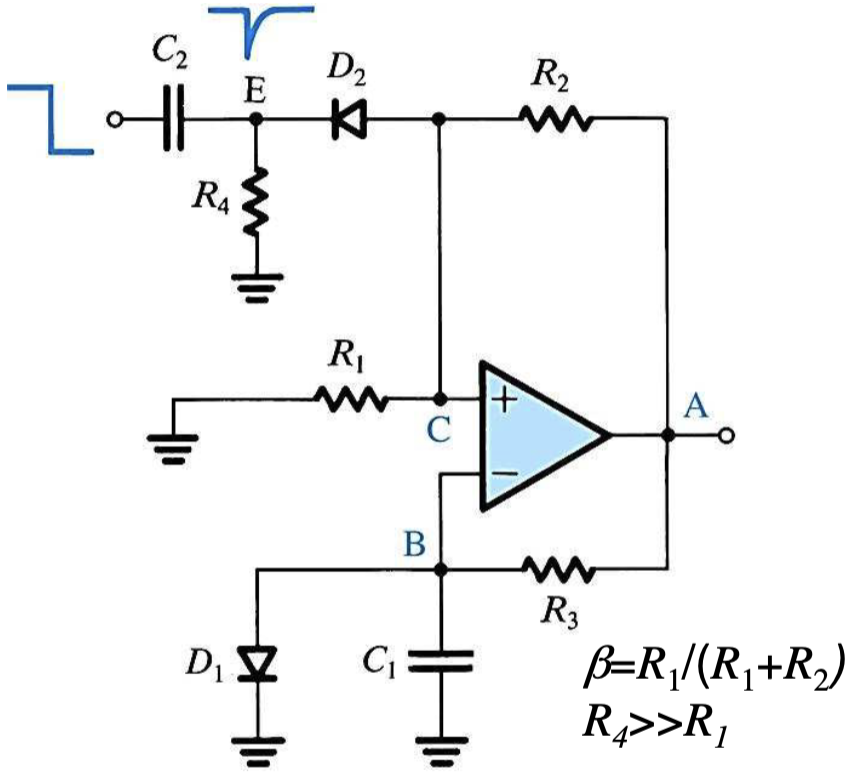
\includegraphics[width=0.8\textwidth]{images/monostable_multivibrator.png}
    \end{center}
    $\ds T = C_1 R_3 \ln \left(\frac{V_{D1} - L_-}{\beta L_- - L_-}\right) \approxeq C_1 R_3 \ln \left(\frac{1}{1-\beta}\right)$
  }

  \formbox{Monostable Multivibrator -- Min Trigger Voltage}{
    \center
      $v_{t, \text{min}} = \beta L_+ - V_{D2} + V_{D1}$
  }

  \formbox{Monostable Multivibrator -- Recovery Time}{
    \center
    $v_B = L_- - (L_- - V_{D1})e^{-t/(C_1R_3)}$\\
    \raggedright
    Setting $v_B= V_\text{diode}$, one can solve for the \textit{recovery time}.
  }

  \formbox{Non-Ideal Inverting Opamp Gain}{
    \centering
    $\ds G = \frac{-\frac{R_f}{R_\text{in}}}{1 + \frac{ \left(1 + \frac{R_f}{R_\text{in}}\right) }{A}}$
  }

  
  
  
\end{multicols*}



\end{document}
